\chapter{Optimizations}
\label{ch:optimizations}

Building a compiler can be likened to building a bridge between
    two distant points.
The semantic gap between your starting point and end point imply the
    complexity of the structure needed to bridge the gap.
Optimizations are the building blocks of such a structure.
If one chooses an input representation sufficiently close to
    the target representation compilation is relatively straight forward
    and often little to no optimization is needed.
Unfortunately as the semantic gap and complexity are inextricably linked
    and as it grows so does the difficulty of writing effective optimizations.
It is not sufficient for a compiler author to be able to perform an
    optimization by hand but they must be able to generalize it into
    a repeatable, inductive process.
The challenge introduced by using a sufficiently abstract and high-level
    representation is designing the transformations and optimizations
    to get us to our end goal.
Given that our goal is state-of-the-art performance in competitive
    area, it is critical we get our optimizations right.
Over the course of my PhD thesis we have designed more than 50 passes
    for Relay, enabling TVM to reach state-of-the-art performance
    on numerous real world models~\citep{huggingface_octoml}.
This chapter focuses on the design and implementation of selected passes.
The remainder of which exist in Apache TVM's source tree
  and are open to all to read and inspect.

\section{Operator Fusion}
\label{sec:fusion}

Operator fusion is an indispensable optimization in deep learning compilers.
Fusion enables better sharing of computation, removal of
  intermediate allocations, and facilitates further optimization by
  combining loop nests.
Fusion is known to be the most critical optimization in machine
  learning compilers, but existing fusion techniques
  are closed (working over a fixed set of ops)
  and target-dependent.
Traditional operator fusion algorithms resemble instruction
  selection:
A sequence of operators eligible
  for fusion is first identified and then replaced with a corresponding
  handwritten fused implementation, usually from a vendor-provided library.
For example, if a fused implementation for a GPU operator does not exist in CuDNN,
  it will remain unfused.
More advanced strategies, implemented in XLA, detect a
  closed set of statically shaped operators for fusion and
  generate code for CPU/GPU.

Relay's fusion algorithm addresses weaknesses of previous approaches by representing
  \textit{all} operators in a secondary IR.
Relay operators are backed by a TVM compute expression that
  describes operations in a high-level DSL that resembles Einstein notation
  but omits low-level scheduling details.
TVM's separation of compute and scheduling provides many favorable qualities
  for Relay's fusion algorithm.
It enables producing shape-specialized fused operators for an open set of operators,
  fusing arbitrary-length chains of operators (not just pairwise combinations),
  and handling operators with multiple outputs and nonlinear consumer-producer patterns.
TVM is also able to reschedule after fusion and perform further optimization via auto-tuning.
Relay performs fusion in two steps, detailed below.

\section{Extraction}

First, Relay identifies subexpressions containing
  fusion-eligible operators and factors them into local functions that
  are marked as primitive.
Primitive functions can later be lowered to platform-specific
  code.
Fusion-eligible subexpressions are identified by constructing a
  directed acyclic graph (DAG) representing data flow between operators.
As the dataflow DAG is acyclic, it allows for the simple construction
  of a post-dominator tree.
Subexpressions are grouped into equivalence classes
  determined by their immediate post-dominator.
The use of the post-dominator tree enables fusion
  between non-linear producer-consumer relationships;
  for example, Relay can fuse diamond-shaped data-flow relations,
  where an input is used by multiple parallel operator chains
  that are combined again by a later operator.
Finally, Relay constructs an expression from each equivalence class,
  collects the expressions' free variables,
  constructs a function with the expression as the body and the free variables
  as parameters,
  and marks it as primitive.
  % TODO add fusion diagram back

\section{Lowering}

In a second step, the Relay compiler converts the generated primitive
  function into platform and shape specific code.
For each operator, Relay collects the high-level \tvm expression that represents it,
  then combines them into an aggregate expression that represents the fused operation.
Generating code using \tvm also requires producing a schedule.
It is possible to use \tvm's default schedule to generate code for a single operation,
  but the default schedule does not support fusion.
In order to generate code for the combined expression, we must generate a
  master schedule based on the set of operations being fused.
The fusion algorithm analyzes the expressions to select a master
  schedule, the master schedule will perform the appropriate scheduling
  actions to generate fused code, such as inlining loops, or reorganizing
  computation.
By combining the master schedule with the fused computation,
  Relay is able to produce an optimized version of the operator
  for any platform supported by TVM.
For example, a related project by one of the co-authors implemented
  a RISC-V backend which immediately obtained full operator fusion
  with no new code.
Due to the Relay compiler's integration with AutoTVM, we can further
  optimize fused operations by performing auto-tuning on the master
  schedule template to obtain the best performance.

\section{Generic Quantization Framework}
\label{sec:quant}

Deep learning is constrained by memory, compute, and accuracy.
Accuracy is often the only metric optimized by machine learning
  researchers, leading to compute- and memory-hungry models.
The sheer number of parameters and the requisite compute
  makes deploying models to resource-limited devices,
  such as in mobile or IoT, challenging.
Even in non-edge devices, the compute cost of using
  datatypes like FP32 is large and computing with mixed precision
  or reduced precision can aid performance.
 An emerging area in deep learning is performing training and inference on
  non-standard numeric types to improve throughput and memory usage.
For example, a single neural network may have more than one million floating-point values
  as its parameters.
The sheer quantity of parameters and their datatypes may limit the ability
  to execute these networks on hardware accelerators.
Accelerators often support fixed point or other non-standard datatypes, at lower precision.
In order to target these devices, Relay must map the computation
  to the appropriate domain.
Unfortunately, reducing bit-width is not a silver bullet and
  can dramatically harm model accuracy.
The tradeoffs between these quantities has lead to the study of quantized neural networks,
  the process by which NNs are modified to use a smaller precision
  or non-standard datatypes to improve throughput and memory usage.
Quantization is particularly essential for supporting many accelerators due to
  their restricted set of datatypes.

State-of-the-art work on quantization suggests that there exist a number of tradeoffs
  between different quantization techniques,
  with the best often determined by platform and model type~\citep{krishnamoorthi18}.
Current deep learning frameworks support a limited number of quantization schemes, and options
  because quantization requires framework support in the form of custom platform-specific operators.
Importantly, there are many different choices of quantization mechanisms.
Each type of quantization has different running time and accuracy properties depending
  on the model as well as the target hardware.
Existing frameworks manually choose a fixed quantized data format, which might be
  suboptimal.
Instead, Relay includes a generic, compiler-based quantization flow that supports a diverse set
  of quantization mechanisms and automatically generate code for each of them.
Relay's generalizable and flexible quantization workflow
  can support customization in both standard devices and acceleration schema
  and address various constraints across different hardware platforms.
The pipeline that we designed can compress and accelerate neural networks with
  low-precision quantization to enable running the deep learning models on edge devices.
Users can overload Relay's existing quantization rewriting rules or add new ones
  to implement different quantization strategies, enabling users to choose between
  signed or unsigned integers or different rounding strategies, such as
  floor, ceiling, or stochastic rounding.

\begin{figure}[h]
  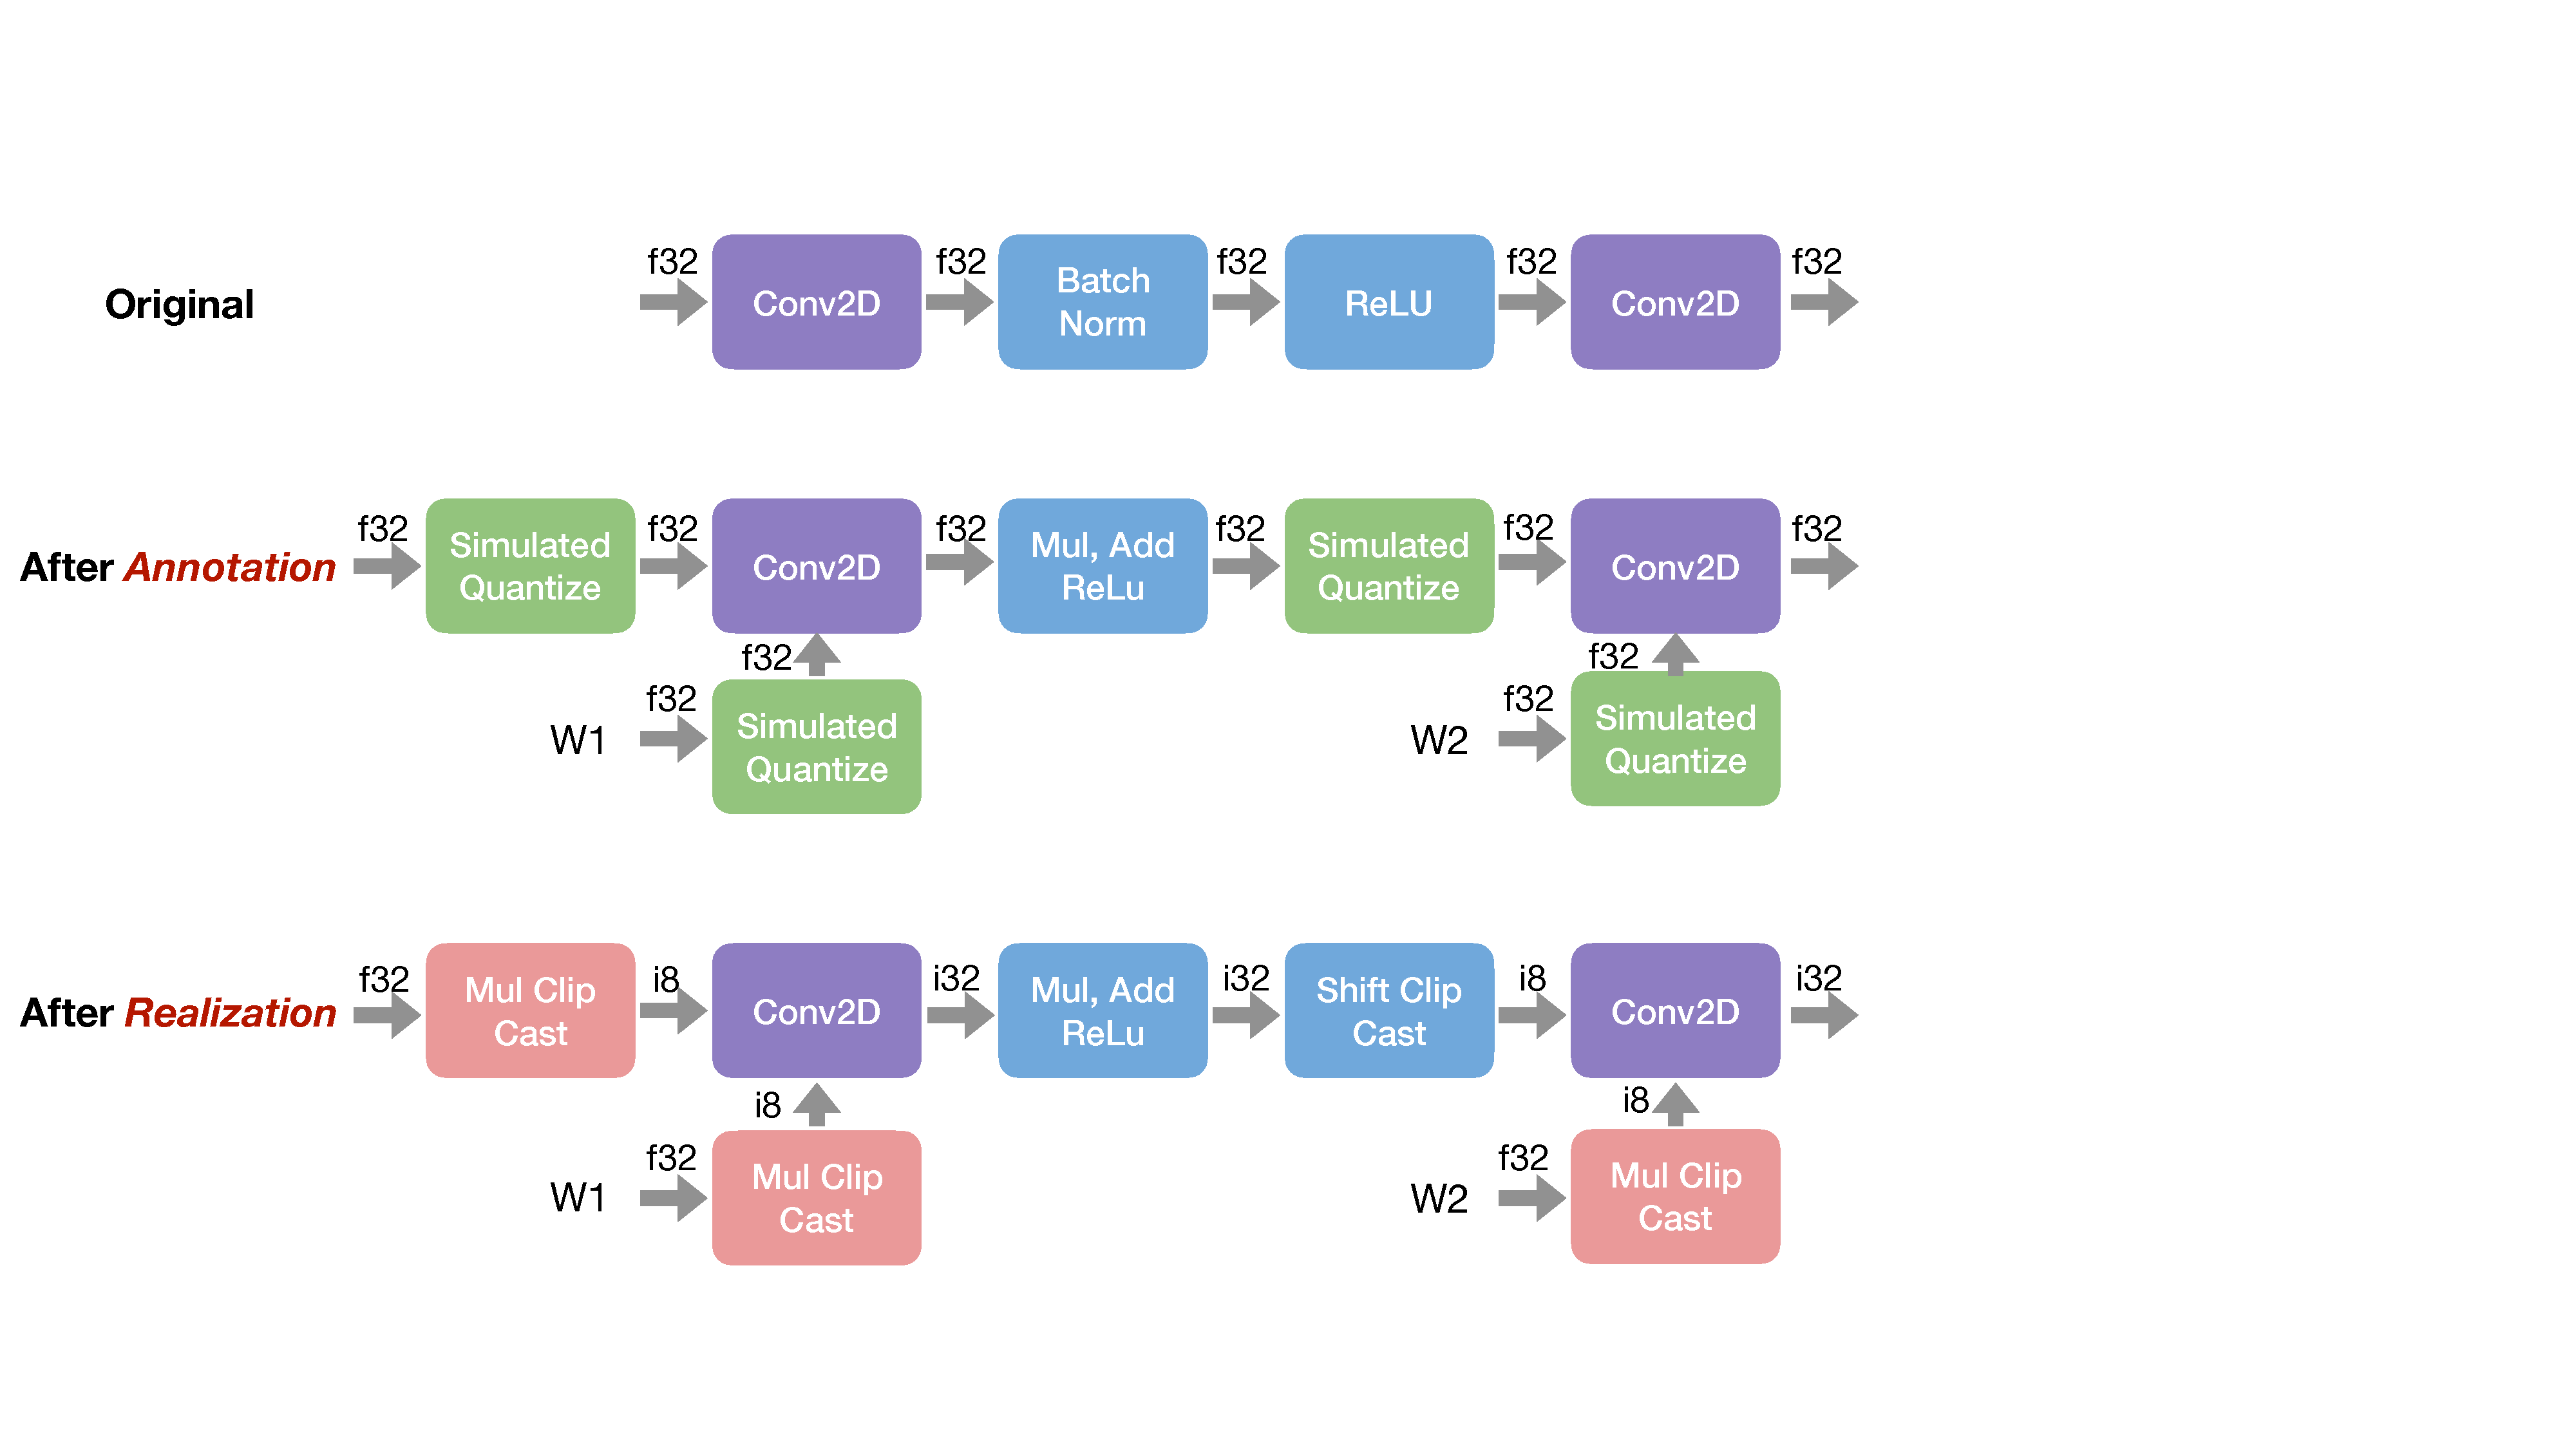
\includegraphics[height=5cm]{fig_splash19/quantization/quant_pdf.pdf}
  \caption{The top graph represents the dataflow graph of operators after annotation,
  and the bottom graph represents the transformed graph.
  SimQ simulates the rounding error and saturating error of quantizing.
  Its argument will get tuned during calibration.}
  \label{fig:quant_flow}
\end{figure}

\begin{figure}[h]
    \begin{equation}
      \begin{aligned}[b]
        \scriptscriptstyle
        & Q(x, r, bit, sign) =\\ & cast(clip(round(x/r*2^{bit-sign}), int8)) \\
      \end{aligned}
    \end{equation}
    \caption{The quantization operation.}
    \label{fig:quant_op}
    \begin{equation}
      \begin{aligned}[b]
        \scriptscriptstyle
        & sim\mathcal{Q}(bits, sign, range) =\\ & \dfrac{clip(round(\dfrac{x}{r} * 2^{bit - sign})) * r}{2^{bit - sign}}
      \end{aligned}
    \end{equation}
    \caption{The simulated quantization operation.}
    \label{fig:sim_quant_op}
\end{figure}

The generic quantization flow proceeds in three steps: annotation, calibration, and realization. We
can apply this pass to convolution-like operators which have a quantized schedule
available. Figure \ref{fig:quant_flow} shows a graphical visualization for this.

\paragraph{Annotate}

Annotation rewrites the program by inserting simulated quantization operations a
  according to an annotation rule of each operator.
The annotation rule describes how to transform an unquantified operation
  into a quantized one.
Each input or output to be quantized is passed to \texttt{sim$Q$},
  an operator that simulates the effect of quantization (for example, from a 32-bit
  floating point value to an 8-bit integer value).

See the definition of simulated quantize, as in Figure \ref{fig:quant_flow}.
We annotate the inputs to this operation with an operator $sim\mathcal{Q}$,
  which simulates the effect of quantization (for example, from a 32-bit
  floating point value to an 8-bit integer value).
However, it is computed with a 32-bit float data type, which is convenient for the
  calibration pass and debugging.
$sim\mathcal{Q}$ has a set of parameters that must then be calibrated in order to
correctly quantize the graph, namely the bits, the scale, and the range.
Finally, after the algorithm has selected
  appropriate setting for these parameters, it applies realization,
  which transforms the simulated quantization operator into the numerator.

% By computing on the unquantized type, Relay can later calibrate the parameters to
%   \texttt{sim$Q$} a necessary step to preserve accuracy of the model.
% \[
%   \texttt{sim$Q$}\left(x, \beta, \sigma, \rho\right) = \dfrac{\texttt{clip}\left(\texttt{round}\left(x / \rho \cdot 2^{\beta - \sigma}\right)\right) \cdot \rho}{2^{\beta - \sigma}}
% \]

\subsection{Calibrate}
The simulated quantized operations have a set of parameters which must
  be calibrated in order to correctly quantize the graph to achieve the
  minimal decrease in accuracy.
As seen above \texttt{sim$Q$} has an input $x$, as well as a number of parameters
  $\beta$, $\sigma$, and $\rho$.
\texttt{sim$Q$}'s parameters control the mapping between the quantized and unquantized type
  and must be calibrated, without calibration the model can be wildly inaccurate.
We must perform an auxiliary optimization task to find the appropriate
  setting for these parameters.
The Relay compiler supports a variety of strategies for setting these
  parameters.
The first strategy implemented is a hyper parameter sweep of a
  single global scale until such a scale is found that does not result
  in overflow.
Another approach is a vision specific scheme which uses
  a per-channel scale, and optimizes the scales using a
  simple mean-squared error loss.
Finally an approach adopted from MxNet uses a
  KL-divergence based loss to optimize the
  quantization scales.

\subsection{Realize}

\begin{table*}[t]
  \begin{tabular}{|c|c||c|c||c|c|}
    \hline
    \multicolumn{2}{|c}{\textbf{ResNet-18}} & \multicolumn{2}{c}{\textbf{MobileNet V2}} & \multicolumn{2}{c|}{\textbf{Inception V3}} \\
    \multicolumn{1}{|c}{Quant.}    & \multicolumn{1}{c}{Accuracy}   &  \multicolumn{1}{c}{Quant.}  & \multicolumn{1}{c}{Accuracy}  & \multicolumn{1}{c}{Quant.}  & \multicolumn{1}{c|}{Accuracy} \\
    \hline
    \texttt{float32} & 70.7 \%    & \texttt{float32} & 70.9 \%       & \texttt{float32} & 76.6 \% \\
    8/16         & 69.4 \%    & 8/32         & 66.9 \%       & 16/32        & 76.6 \% \\
    8/32         & 69.4 \%    & 8/16         & 66.9 \%       & 8/32         & 75.2 \% \\
    \hline
  \end{tabular}
  \caption{This table shows the accuracy of various quantized models.
    \texttt{float32} refers to the non-quantized model.
    Notation as in ``8/16`` refers to 8-bit quantization,
    16-bit accumulation}
  \label{fig:quant_results}
\end{table*}

The realization pass transforms the simulated quantized graph
  (which uses 32-bit floats)
  into a real low-precision computation graph.
The simulated quantized operator is transformed
  into several fine-grained operations like multiplication and addition.
This transforms the \texttt{sim$Q$} operator into the below quantization operator.
\[
  Q\left(x, \rho, \beta, \sigma\right) = \texttt{cast}\left(\texttt{clip}\left(\texttt{round}\left(x / \rho \cdot 2^{\beta-\sigma}\right), \texttt{qtype}\right)\right)
\]
Due to Relay's handling of fusion
  we are able fuse these scaling operations directly into
  to the original operator, transforming a convolution
  from \verb|fp32| to a type such as \verb|int4|.

To avoid the overflow, it also would be better to use larger global scale.
 With flexible configure, our workflow can be customized as best strategy for
 different networks and hardwares.
Quantized models require low-precision operators for efficiency. Due to our operator representation,
and the ability to leverage AutoTVM, TVM's auto tuner, we can automatic generate kernels for arbitrary
types without effort.

\begin{figure}[t]
  \begin{minted}[fontsize=\footnotesize]{python}
  @register_annotate_function("nn.conv2d", override=True)
  def annotate_conv2d(ref_call, new_args, ctx):
      lhs, rhs = new_args
      lhs = attach_simulated_quantize(lhs, sign=False, rounding='round')
      rhs = attach_simulated_quantize(lhs, sign=False, rounding='stochastic_round')
      return expr.Call(ref_call.op, [lhs, rhs], ref_call.attrs)
  \end{minted}
  \caption{
    An example of overloading the annotation function for 2-d convolution.
    In this example we treat both input, and the weights as unsigned integers,
    applying rounding to the input, and stochastic rounding to the weights.}
  \label{fig:annotate_conv}
\end{figure}

Developers can customize quantization with very little code.
For example, the quantization annotation function may be overloaded for any operation,
  making use of signed or unsigned integers, or different rounding strategies, such as
  floor, ceiling, or even stochastic rounding (Figure~\ref{fig:annotate_conv}).

To demonstrate the effectiveness of our generic quantization,
  we use Relay to explore
  different choices of input and accumulation bits.
The results are shown in Table~\ref{fig:quant_results}.
We find that no single strategy fits all use cases.
For certain network architectures such as MobileNet and ResNet, 16-bit to 32-bit
  quantization provides good accuracy,
   but 8-bit to 16-bit provides the best speedup,
  assuming the input does not overflow.
The current framework demonstrates the importance of applying
  various quantization schemes based on networks and hardware platforms.

\subsection{Quantized Inference on ARM Platforms}
To demonstrate the effectiveness of our generic quantization (see Section~\ref{sec:quant}),
  we use Relay to evaluate both \textit{accuracy} and \textit{performance} of different
  quantization schemes on vision workloads.
To evaluate \textit{accuracy},
  we tested various quantization schemes
  (denoted $m/n$ for $m$-bit quantization and $n$-bit accumulation)
  against a \texttt{float32} baseline on three vision models,
  as shown in the table below:
\begin{center}
  \begin{tabular}{|c|c||c|c||c|c|}
    \hline
    \multicolumn{2}{|c}{\textbf{ResNet-18}} & \multicolumn{2}{c}{\textbf{MobileNet V2}} & \multicolumn{2}{c|}{\textbf{Inception V3}} \\
    \multicolumn{1}{|c}{QS}    & \multicolumn{1}{c}{Acc.}   &  \multicolumn{1}{c}{QS}  & \multicolumn{1}{c}{Acc.}  & \multicolumn{1}{c}{QS}  & \multicolumn{1}{c|}{Acc.} \\
    \hline
    \texttt{fp32} & 70.7 \%    & \texttt{fp32} & 70.9 \%       & \texttt{fp32} & 76.6 \% \\
    8/32         & 69.4 \%    & 8/32         & 66.9 \%       & 16/32        & 76.6 \% \\
    8/32         & 69.4 \%    & 8/16         & 66.9 \%       & 8/32         & 75.2 \% \\
    \hline
  \end{tabular}
\end{center}
Figure~\ref{fig:portability-eval} shows the results of different
  levels of quantization on \textit{performance} when applied to the Raspberry Pi 3
  and Firefly RK3399 ARM-based platforms.
The numbers show that as we opt for a more aggressive quantization scheme
  (e.g., 8/16),
  we achieve much improved performance with hardly a drop in accuracy.
Interestingly,
  on some model/platform pairs,
  the \texttt{int8/int32} scheme performs slightly worse than \texttt{float32} on both platforms,
  which likely stems from the existence of faster hardware intrinsics for 16-bit operations on these systems.

\section{Partial Evaluator}
\label{sec:t formartial_eval}
Existing deep learning IRs have relied on
  a mixture of staging and constant evaluation
  in order to optimize user programs.
Partial evaluation is a generalized form of constant
  evaluation that can reduce partially constant
  programs.
A partial evaluator (PE) allows the use of high-level abstractions
  without limiting code that \textit{could} in practice be
  compiled to a particular target.
Relay is the first compiler to apply partial evaluation
  techniques to deep learning, the
  core approach of which is based on \citep{pe_ref}.
Partial evaluation, when composed with other
  optimizations like fusion, yields a variety
  of useful optimizations without requiring
  a separate implementation of each.
For example, the partial evaluator can be used to perform
  loop unrolling, which then enables further fusion,
  without any additional compiler passes.
We describe the implementation and some
  concrete applications of partial evaluation
  in Chapter~\ref{ch:ad}.

\section{Dynamic Memory Allocation, Device Placement, and Code Generation}

A key challenge preventing existing deep learning compilers from handling dynamism
  is the lack of a uniform and dynamic representation.
For example, optimizations and runtime of existing IRs,
  e.g., TVM's NNVM~\citep{tvm_osdi18} assume the presence of static shape information.
These assumptions introduce quite a few challenges for optimizing dynamic behaviors.
This section describes how we transform standard TVM programs into our dynamic dialect
  which enables us to easily apply static optimizations to dynamic programs, much as we
  do in traditional compiler optimization.
Particularly, we detail three key components required to compile dynamic models.

\begin{itemize}
    \item An extended type system which enables static tracking of dynamic shapes.
    \item A series of optimization passes that make dynamic output shapes, allocation,
          and device placement explicit.
    \item A set of code generation techniques for producing code of kernels with dynamic input
          and output shapes.
\end{itemize}

\subsection{Dynamic Memory Planning}
\label{subsec:optimizations:memory}

Deep learning workloads are dominated by two key factors
  (1) compute-intensive kernels and (2) memory consumption and allocation.
Many deep learning compilers employ a form of static memory planning which
  tries to coalesce memory allocations and minimize memory consumption.
For devices such as GPUs these optimizations are essential for reducing
  memory fragmentation and ensuring allocation does not hamper kernel performance.
Existing deep learning compiler IRs hide memory allocation behind a functional interface,
  where each operator implicitly allocates their output storage.
Then before execution, the system performs static-memory planning on the
  data-flow graph enabling efficient pre-allocation of the required memory.
Due to this ``out-of-band'' nature of memory allocation,
  it is challenging to customize, modify or compose memory optimizations with other passes.
For example, if one needs to adjust memory allocation for heterogeneous execution,
  modifications to the runtime are required.
TVM's graph runtime is one such example of static memory planning.

Alternatively, some systems lower the entire program to low-level IRs such as
  LLVM~\citep{llvm} in order to perform optimizations.
Due to the coarse-grained memory semantics of deep learning models,
  it is essential that memory optimizations occur at a suitably
  high-level of abstraction before essential program facts are lost.
Moreover, as discussed in~\autoref{sec:compilation:shape-func},
  we have introduced new ways to account for the handling of dynamic allocations,
  which further complicate memory analysis.
In order to perform dynamic memory planning we have extended Relay's IR with
  a set of new primitives we dub the ``memory dialect''.
The memory dialect is a subset of Relay programs where all memory allocations are
  explicit.
The key to this transformation is an inter-procedural change of calling convention,
  with each operator now taking its outputs explicitly it is possible to
  track and transform allocations.
In particular, we have introduced four new IR constructs,
  (a) \verb|invoke_mut(op, inputs, outputs)| which takes outputs as mutable in-out arguments,
  (b) \texttt{alloc\_storage(size, alignment, device)} which allocates a region of memory
      of a particular size,
  (c) \texttt{alloc\_tensor(storage, offset, shape, dtype, attrs)} which allocates
    a tensor at a particular storage offset
    with a shape and data type, and
  (d) \verb|kill(tensor)| which frees a tensor before its reference count
    becomes zero due to exiting the frame.
Note that in the below code examples \texttt{Tensor<d1, ..., dn>}
is shorthand for a tensor of shape \texttt{(d1, ..., dn)} containing floating point values.

We can demonstrate how to transform a single statically shaped operation such as broadcasting addition.

\begin{minted}{rust}
fn main() -> Tensor<10> {
  let t1, t2 : Tensor<10> = ...;
  add(t1, t2)
}
\end{minted}

Here we only must allocate a single buffer, the return buffer for the addition operation.

\begin{minted}{rust}
fn main() -> Tensor<10> {
  let t1 = ...; let t2 = ...;
  let storage = alloc_storage(40, 64, cpu(0));
  let out1= alloc_tensor(storage, 0, (10), f32);
  invoke_mut(add, (t1, t2), (out1));
  out1
}
\end{minted}

The above transformation replaces all operator invocations with a call to
  \verb|invoke_mut|, a corresponding allocation of backing storage, and a single
  tensor placed at offset zero.
The key insight is to internalize a notion of memory allocation into the IR,
  enabling static optimization of both static and dynamic allocations presence of
  control and dynamic shapes.
We realize our shape functions as fragments of TVM's tensor expression language
  which computes the output shape for a particular operator.
As detailed in~\autoref{sec:compilation:shape-func} our shape functions
  may require the input, the input \textit{shape}, or both.
Our uniform treatment of shape functions as standard tensor expressions enables them
  to be fused and optimized like normal, but one challenge is that we must now manifest allocations
  in a fixed point until we allocate for both the compute and necessary shape functions.
We illustrate this below with a single dynamic concatenation.

\begin{minted}{rust}
fn (x: Tensor<?,2>, y: Tensor<1,2>)->Tensor<?,2> {
  concat((%x, %y))
}
\end{minted}

This is the same transformation as the previous example with the addition of carefully inserting
invocations to the shape function to compute output buffers sizes for the dynamically sized kernel.

\begin{minted}{rust}
fn (x: Tensor<?,2>, y: Tensor<1,2>)->Tensor<?,2> {
  let in_sh0 = shape_of(x);
  let in_sh1 = shape_of(y);
  let storage_0 = alloc_storage(16, 64, ...);
  let out_sh0 = alloc_tensor(storage_0, ...);
  invoke_shape_func(concat,
      (in_sh0, in_sh1), (out_sh0,), ...);
  let storage_01 = alloc_storage(...);
  let out_0 = alloc_tensor(
      storage_01, shape_func_out_0, ...);
  invoke_mut(concat, (x, y), (out_0));
  out_0
}
\end{minted}

After the transformation you may notice we have introduced calls to \verb|shape_func| which
  invokes a shape function corresponding to the kernel.
The shape function requires input shapes as arguments which further require us to invoke \verb|shape_of|
  for both \verb|%x| and \verb|%y|.
\verb|shape_of| will be directly mapped to a VM instruction to retrieve the shape of a tensor at runtime.
More description of it will be provided in \autoref{sec:compliation:hetero}.

Now that the all allocations are explicit in the IR we can provide analogous
  optimizations in the static case on dynamic programs,
  for example we have implemented a storage coalescing pass which groups storage
  into a larger region which we can then multiplex tensor allocations on to.

The key insight is to internalize a notion of memory allocation into the IR,
  enabling static optimization of both static and dynamic allocations in the presence
  of control and dynamic shapes.
Now that all allocations are explicit in the IR, we can provide analogous optimizations
  in the static case on dynamic programs, for example we have implemented a storage coalescing
  pass to group storage into a larger region which allows the multiplexing of multiple tensor
  allocations to a single piece of storage.
Further optimization like liveness analysis and graph coloring algorithm can be applied to
  the program to reuse storage.

\subsection{Heterogeneous Device Placement}
\label{sec:optimizations:hetero}

As discussed in Section \autoref{sec:compilation:shape-func}, shape functions are executed at runtime to
  calculate the output shape of an operator.
These functions must execute on the CPU due to the host-interaction model of GPU like devices.
In the case of heterogeneous execution (i.e., CPU and GPU) it is essential to carefully schedule
  the execution of shape functions and kernels as improper scheduling creates memory copies
  which can be disastrous for performance.
For instance copying the inputs to shape functions from the GPU results
  in considerable performance penalty.
To minimize overhead we analyze allocations and memory transfers so we can place
  each sub-expression on the correct device.

We introduce a unification based analysis for computing the correct device placement and
  allocation based on the previous scheduling of the compute kernels.
The goal of our device analysis is assigning each IR node in a way that minimizes
  the number of cross-device copies. We introduce a concept of \texttt{DeviceDomain}
  to represent the domain of a device, including source and destination.
Each expression in the IR defaults to the empty domain, meaning there
  are no constraints on its device placement.
In addition, two new IR constructs are introduced to facilitate the heterogeneous execution of VM,
  namely \verb|device_copy| and \verb|shape_of|.
The former performs a data transfer between different devices and is
  inserted when a cross-device data copy is mandatory.
The latter is used to retrieve the shape of a tensor at runtime and is
  used to efficiently compute the input shapes for shape functions.
Our analysis is formulated as a set of device placement rules which describe how device constraints
  flow, and then we use unification, a technique common in type inference and compilers
  in order to compute precise device placement.

As discussed in \autoref{sec:compilation:shape-func},
  shape functions are executed at runtime to calculate the output shape of an operator.
These functions should execute on the CPU as their outputs are used to compute the size of allocated memory.
In the case of heterogeneous execution (i.e., CPU and GPU),
  it is essential to carefully place the execution of IR nodes to proper devices.
Otherwise, considerable overhead from data transfers and device synchronization will
  occur if the inputs to shape functions and kernels need to be copied from or to GPU.
To minimize the performance penalty, we analyze the program to place sub-expressions on the most suitable devices.

% TODO import rules from appendix.

\begin{itemize}
    \item \verb|shape_of|. Defaults to the CPU domain because we can access a Tensor's shape
                           regardless of which device it is placed on.
    \item Shape functions. These IRs take the output of one or multiple \verb|shape_of| and then derive
                           the shape of an operation according to predefined type inference rules.
                           The output of a shape function is used to compute the amount of memory that this operator
                           requires at runtime, which only needs a few cheap scalar arithmetic computation.
                           Therefore, the inputs and outputs would be better on a CPU domain as well.
    \item \verb|device_copy|. The input and output of this IR are on different domains as it copies data from one domain to another.
                              The device domains of the input and output are propagated in the opposite directions
                                to other IR nodes that are reachable to/from the device copy node.
    \item Memory operations. The device domain of storage from \verb|alloc_storage| is designated in the expression,
          and later is propagated to the device domain of the tensors allocated from this storage via \verb|alloc_tensor|.
          in the instruction computation of the allocation size and the shape for memory operations,
          such as \verb|alloc_storage| and \verb|alloc_tensor|, should be on CPU due to low computation intensity.
    \item \verb|invoke_mut|. All arguments used in the \verb|invoke_mut| must have the same device domain.
    \item Other common IR nodes. The device domain of other common IR nodes,
            e.g. variables, constants, operators, etc., can be directly propagated from the above nodes.
\end{itemize}


\begin{figure}
    \centering
    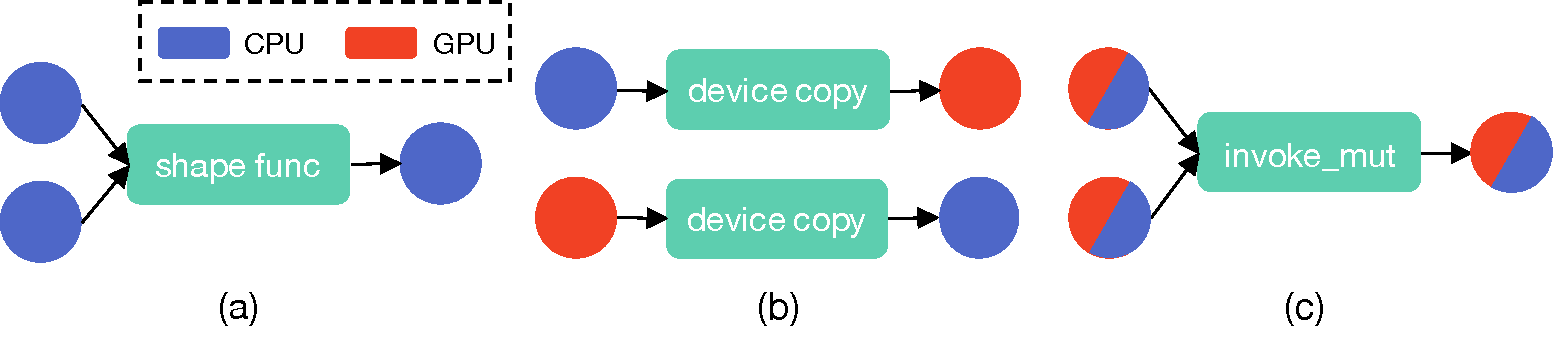
\includegraphics[width=\linewidth]{figs/hetero.pdf}
    \caption{Some heterogeneous device placement rules. (a) The inputs and outputs of shape functions are placed on CPU.
    (b) \texttt{device\_copy} changes the device of output accordingly.
    (c) The device of all arguments to \texttt{invoke\_mut} must be the same.
    }
    \label{fig:hetero}

\end{figure}

Based on the rules defined above, we use a union-find data structure to bidirectionally
  propagate and unify the device placement of each IR node.
We introduce two operations, \texttt{union(s, t)} and \texttt{find(s)},
  to achieve \texttt{DeviceDomain} unification throughout the entire program.
\texttt{union(s,t)} unions the equivalence device domains of \texttt{s} and \texttt{t}
  into one equivalence domain when the device types match.
\texttt{find(s)} returns the representative of the device domain
  that \texttt{s} belongs to.
These two operations are applied until all IR nodes are annotated.
The result of the heterogeneous device placement composes with memory planning
  and shape function insertion resulting in correctly placed allocations.

\subsection{Dynamic Kernel Code Generation}
\label{sec:compliation:codegen}

Deep learning compilers~\citep{tvm_osdi18, halide} have demonstrated competitive performance
  compared to manually tuned kernels on multiple platforms.
Recent trends apply machine learning based search to further reduce
  or eliminate complex manual performance tuning,
  existing work applies both template based~\citep{chen2018learning, zheng2020flextensor}
  and beam search based~\citep{adams2019learning} ones.

However existing work which focuses on tuning in the presence of fully
  static shape information falls short in the presence of symbolic or dynamic shapes.
There are two inherent challenges with regards to performing code generation for symbolic shapes.
\begin{itemize}
    \item How to achieve the same performance of kernels generated with symbolic shapes as
          that with static shapes when applying the same schedule?
    \item How to extend the machine learning based auto-tuning to kernels with symbolic shapes?
\end{itemize}

Loop parallelism and loop tiling are common optimization techniques that exploit multi-core capabilities
  by achieving data access patterns which are memory hierarchy aware for both CPUs and GPUs.
However, the combination of these techniques often introduce complex loop boundary conditions.
In many static cases, it is possible to prove these conditions always hold,
  and thus eliminate checks which hamper further optimizations such as unrolling.
While straightforward to handle with static shapes, it becomes a non-trivial challenge
  when performing symbolic code generation.
If not carefully handled, the boundary condition checks will stay, leading to poor performance.

To address this issue, we generate multiple kernels according to the residues modulo of the tiling
  factor and then dispatch based on the actual shape at runtime.
For example, suppose a symbolic dimension $x$ is divided by a factor of 8, we then
  generated eight duplicated kernels replacing the symbolic var $x$ by $8k+r$ in each copy,
  where $k = \lfloor x / 8 \rfloor$ and $r \in [0..7]$.
Lastly, we automatically generate a dispatch function which invokes
  the corresponding kernel based on the residue.
By applying this technique in conjunction with an enhanced symbolic expression simplification pass,
  we can eliminate most boundary checks to achieve performance that is nearly identical
  to kernels compiled with a single static shape.
Lastly, we automatically generate a dispatch function that invokes the
  corresponding kernel based on the residue.
This strategy can be viewed as a form of polymorphic inline caching~\citep{inline_caches},
  where the cache is not keyed by type, but shape.
Both the dispatch logic and kernels are represented as TIR code enabling them
  to be optimized and compiled using standard mechanisms.

In addition, the dispatch function can be extended to invoke either compiler generated kernels
  or third party library whichever is faster from the profiling results.
The increased kernel size is relatively small compared to the overall deep learning models.
In extreme cases where resources are extremely limited,
  we can either generate fewer number of kernels than the tiling factor
  or reduce the tiling factor to find an acceptable trade-off
  between code size and performance.
In case where resources are extremely limited, we can either generate fewer number of kernels
  than the tiling factor or reduce the tiling factor to find an acceptable
  trade-off between code size and performance.

A known issue to machine learning based tuning is that it may take a long time (usually hours) to find
  the best schedule for a single kernel.
When it comes to symbolic shapes, the tuning time may be exponentially longer if we
  naively tune for every possible shape.
In this paper, we extend the template based tuning approach for
  symbolic shapes in order to make tuning time tractable.
The template based tuning approach takes a human-defined
  code template and a search space, and searches the best configure
  within the search space by using machine learning algorithms.
We observe that a good configuration for one shape usually performs
  well on other shapes.
Based on this observation, we devise the following mechanism
  to tune the kernel for symbolic shapes.

\begin{enumerate}
    \item First replace the symbolic dimensions by a large enough value (e.g., 64) such that the search space can cover most possibilities, and run the tuning algorithm on the static shape for a sufficient number of iterations.
    \item Pick top $k$ configurations, apply them to a selection of other shapes, and evaluate their performance.
    \item Pick the configuration that performs best on average among shapes previously evaluated.
\end{enumerate}

We found that $k=100$ covers most of the best configurations for other shapes.
Current popular dynamic models usually only require kernels with one symbolic variable.
As a result, we choose the values of power of two up to 256 in the cross evaluation of other shapes.
If there is more than one symbolic variable, a more sophisticated selection approach might be
  required to limit the evaluation time of step 2.
We leave this to the future work.
Further, if the workload distribution is known, we could adjust the weighting
  of known shapes when picking the best configuration for step 3.

Though we address both challenges, we admit that our approach has limitations when
  all dimensions are unknown.
In these cases symbolic codegen cannot completely replace manually tuned 3rd party libraries yet,
  but is complimentary when partial shapes are known.

\section{Accelerator-Specific Optimizations}
\label{sec:accel-opts}

Many accelerates provide non-traditional programming
    abstractions to compilers and users.
For example many traditional platforms can have
    code generated via LLVM.
These simply expose an LLVM backend which generates
    a well known ISA.
Many accelerators are not programmable in this style
    and require a mixture of driver interactions
    and static and dynamic code generation to
    drive a program to completion.
Even on very popular accelerators such as GPU
    violate the typical CPU programming model.
In order to lower generic deep learning programs
    to these types of accelerators it is
    essential we are able to optimize programs.
For example some accelerators only support
    low-bit datatypes converting quantization
    from an optimization to a necessary program
    transformation.

Although DL accelerators form a diverse family of designs,
  one property they have in common is a restricted computing model.
The consequence of this is that individual accelerators
  can rarely execute entire Relay programs.
For example, some accelerators cannot execute unbounded loops,
  requiring individual computations to be scheduled via
  host device (often a CPU) which interacts with the device runtime
  as well as programming it.

Below we highlight a few of these optimizations that were used
  to implement support for the VTA~\citep{moreau2018vta} accelerator
  discussed in Chapter~\ref{ch:execute}.

\textit{Axis scale folding} is an optimization that removes scaling
  operations that occur before or after convolution-like operators.
The multiplication by a scalar is moved through a convolution towards
  its constant inputs, such as parameters.
By moving the scaling operation to a constant weight, we are able
  to compute away the scale using the partial evaluator.
This optimization is required for certain accelerators that lack scalar multipliers~\citep{moreau2018vta}.
In order to target these accelerators,
  we must eliminate \textit{all} scalar operations.

\textit{Parallel convolution combination} is a specialized
  optimization that fuses multiple 2D convolutions that share the same input.
The goal of this pass is to produce a larger kernel for the GPU,
  as each kernel launch on the GPU has overhead.
It was designed with the Inception network \citep{inception} in mind, as it
  contains blocks of convolutions that share the same input.
The entire parallel convolution combination pass,
  including documentation and tests,
  required fewer than 350 lines of code and was contributed
  by a non-Relay affiliated undergraduate student
  in their first contribution to our codebase.

\section{Dataflow Rewriting}

A key portion of compiler optimization is
  the selection and application of rewrite rules for a variety
  of use cases.
Many of optimizations, especially those around program partitioning can
  be phrased a sequence of rewriting rules over a program or set of
  programs.
We have explored two very different rewriting approaches in TVM
  the first was specifying dataflow patterns for end users to
  match dataflow graph properties and select subgraphs.
The second was the use of Egg TODO a library
  for utilizing equivalence graphs to perform saturated rewriting.
We describe both approaches in the context of the TVM stack
  below.
